\documentclass[oneside]{book} % oneside removes blank pages after new parts.
\usepackage[utf8]{inputenc}
% Enables proper hyphenation and informs other packages of the language this
% document uses.
\usepackage[english]{babel}
% Latin Modern (a font with all the characters).
\usepackage{lmodern}
% AMS stuff
% Proof environment, etc
\usepackage{amsthm}
% Vertical matrices, etc
\usepackage[fleqn]{amsmath}
% Set symbols (N, Z, Q, R, C)
\usepackage{amssymb}
% The \midrule glyph
\usepackage{booktabs}
% To get "not equivalent to"
\usepackage{centernot}
\usepackage{listings}
% Turns off the indentation and adds a little bit of (stretchable) space in
% between paragraphs.
\usepackage{parskip}
\usepackage{graphicx}
\usepackage{wrapfig}
\usepackage{hyperref}
\usepackage{commath}

\theoremstyle{plain}
\newtheorem*{theorem*}{Theorem}

\hypersetup{
    colorlinks=true,  % Colored links.
    linktoc=all       % Link both sections and subsections.
}

\graphicspath{ {images/} }

\DeclareMathOperator\cis{cis} % used for complex numbers
% most of the time, \newcommand* is the best choice as you want the
% error-checking that it provides.
\newcommand*\conj[1]{\bar{#1}}
\newcommand*\mean[1]{\bar{#1}}
\newcommand*\reciprocal[1]{\frac{1}{#1}}
\newcommand*\argument{\phi}
% number sets
\newcommand*\primes{\mathbb{P}}
\newcommand*\naturalnumbers{\mathbb{N}}
\newcommand*\wholenumbers{\mathbb{W}}
\newcommand*\integers{\mathbb{Z}}
\newcommand*\rationalnumbers{\mathbb{Q}}
\newcommand*\irrationalnumbers{\mathbb{I}}
\newcommand*\reals{\mathbb{R}}
\newcommand*\complexnumbers{\mathbb{C}}

\lstset{frame=tb,
	language=Java,
	aboveskip=3mm,
	belowskip=3mm,
	showstringspaces=false,
	columns=flexible,
	basicstyle={\small\ttfamily},
	numbers=left,
	breaklines=true,
	breakatwhitespace=true
}

\title{Formulas}
\author{Bernardo Sulzbach
(\href{mailto:mafagafogigante@gmail.com}{mafagafogigante@gmail.com})}
\date{\today}

\begin{document}

\hypersetup{pageanchor=false} % This prevents a warning.
\begin{titlepage}
\maketitle
\end{titlepage}
\hypersetup{pageanchor=true}


\tableofcontents

\part{Introduction}
This document is a collection of notes and formulas from various subjects I
need to remember. It is mainly for reference purposes.

\part{Chemistry}

\chapter{Gases}

Ideal gas law
\[PV = nRT\]

Diffusion. Diffusion is the rate at which two gases mix.
Effusion. Effusion is the rate at which a gas escapes through a pin hole.

Graham's law of diffusion or effusion

Graham's law states that the rate of effusion or of diffusion of a gas is
inversely proportional to the square root of its molecular weight.

\[\frac{R_1}{R_2} = \sqrt{\frac{M_2}{M_1}}\]

In the same conditions of temperature and pressure, the molar mass is
proportional to the mass density. Therefore the rate of diffusion of different
gases is inversely proportional to the square root of their mass densities.

\[\frac{R_1}{R_2} = \sqrt{\frac{M_2}{M_1}}\]

\chapter{Solutions}

Solution. A solution is a homogeneous mixture of two or more substances.

Solute is a substance that is dissolved in the solution.

Solvent is the substance that dissolves the solute. Solvent is present in
greater amount.

Concentration is the ratio of solute and solvent.

Concentration can be measured using molarity, molality and mole fraction.

\[\text{Molarity (M)} = \frac{\text{moles of solute}}{\text{liters of
solution}}\]

\[\text{Molality (m)} = \frac{\text{moles of solute}}{\text{kg of solution}}\]

Mole fraction. The mole fraction of a component in solution is the number of
moles of that component divided by the total number of moles of all components
in the solution.

\[X_A = \frac{n_A}{\sum{n_x}}\]

Dilution. Diluting a solution means adding more solvent without adding more
solute.
The following formula is quite helpful in these calculations.

\[M_i V_i = M_f V_f\]

Mole. Mole is the amount of substance that contains same number of particles as
there are atoms in 12 grams of pure carbon-12.

One mole of substance is Avogadro's number.

The number of molecules in a mole is known as Avogadro's constant.

\[N_A = 6.023 \cdot 10^{23}\]

One mole of gas has a volume of 22.4 liters at Standard Temperature and
Pressure.

Relation between moles and grams.
One mole of a substance weights the molecular weight of substance in grams.

\chapter{Atomic Properties}

Ionization energy. Ionization energy is qualitatively defined as the amount of
energy required to remove the most loosely bound electron of an isolated
gaseous atom to form a cation. It is always endothermic (positive).

\chapter{Acids and Bases}

The Henderson-Hasselbalch equation describes the derivation of pH as a
measure of acidity (using pKa, the negative log of the acid dissociation
constant).

\[pH = pK_a + \log_{10} \frac{[\text{A}^-]}{[\text{HA}]}\]
\[pOH = pK_b + \log_{10} \frac{[\text{BH}^+]}{[\text{B}]}\]

where [A-] is the concentration of conjugate base and [HA] is the concentration
of the acid.

\chapter{Kinetics}

One of the most important topics of chemical kinetics is the \textbf{rate law}.
The rate law is an expression relating the rate of a reaction to the
concentrations of the chemical species present, which may include reactants,
products, and catalysts. Many reactions follow a simple rate law, which takes
the form
\[v = k [A]^\alpha [B]^\beta \ldots\]
For reactions with multiple steps, the rate law, rate constant, and order are
determined by experiment, and the orders are \textbf{not} generally the same as
the stoichiometric coefficients in the reaction equation.  A final important
point about rate laws is that overall rate laws for a reaction may contain
reactant, product and catalyst concentrations, but must not contain
concentrations of intermediates.

\paragraph{Law of Mass Action.} The law of mass action is a general description
of the equilibrium condition; it defines the \textit{equilibrium constant
expression}.
\[K_C = \frac{[C]^\gamma [D]^\delta}{[A]^\alpha [B]^\beta}\]

\paragraph{Notes on the equilibrium expression.} The equilibrium expression for
a reaction is the reciprocal of that for the reaction written in reverse. When
the equation for a reaction is multiplied by n, \(K\) is raised to n.  The
units for \(K\) depend on the reaction being considered, but it is
\textbf{customarily written without units}.

\paragraph{Equilibrium in terms of pressure.} The equilibrium expression for a
reaction can be written in terms of partial pressures.
\[K_P = \frac{\left(P_C\right)^\gamma
\left(P_D\right)^\delta}{\left(P_A\right)^\alpha \left(P_B\right)^\beta}\]
\[K_P = K_C (RT)^{\Delta n}\]
where

n is the difference between the number of moles of gases in the products and in
the reactants.

\paragraph{Heterogeneous Equilibrium.} The equilibrium constant does not depend
on the amounts of pure solid
or liquids present. Just gases and aqueous solutions are taken into account.

\paragraph{The Reaction Quotient (Q).} In general, all reacting chemical
systems are characterized by their Reaction Quotient, Q. It has the same
formula as K, but can be used even when the system is not at equilibrium.

\paragraph{Le Chatelier's Principle.} \textit{If a system at equilibrium is
disturbed, the system tends to shift its equilibrium position to counter the
effect of the disturbance.}

\chapter{Organic Chemistry}
Organic chemistry is dominated by the functional group approach, where organic
molecules are constructed from an inert hydrocarbon skeleton onto which
functional groups are attached.

The properties and reaction chemistry of a particular functional group are
highly independent of environment. Therefore, it is only necessary to know about
the chemistry of a few functions in order to predict the chemical behavior of
thousands of real organic chemicals.

\section{Alcohols}
\subsection{Primary alcohol}
Primary alcohols have an -OH function attached to an R-CH2- group.

Primary alcohols can be oxidised to aldehydes and on to carboxylic acids.

Primary alcohols can be shown as \texttt{RCH2OH}.

\subsection{Secondary alcohol}
Secondary alcohols have an -OH function attached to a R2CH- group.

Secondary alcohols can be oxidised to ketones.

Secondary alcohols can be shown as \texttt{R2CHOH}.

\subsection{Tertiary alcohol}
Tertiary alcohols have an -OH function attached to a R3C- group.

Tertiary alcohols are resistant to oxidation with acidified potassium
dichromate(VI), K.

Tertiary alcohols can be shown as \texttt{R3COH}.

\section{Diol or polyol}
Diols and polyols are alcohols with two or more -OH functions.

Diols and polyols are very soluble in water. They are used as high temperature
polar solvents.

\section{Aldehydes}
Aldehydes have a hydrogen and an alkyl (or aromatic) group attached to a
carbonyl function.

Aldehydes are easily oxidized to carboxylic acids, and they can be reduced to
primary alcohols.

Aldehydes can be shown as \texttt{RCHO}.

\section{Ketones}
Ketones have a pair of alkyl or aromatic groups attached to a carbonyl function.

Ketones can be shown as \texttt{RCOR}.

\section{Carboxylic Acids}
Carboxylic acids have an alkyl or aromatic groups attached to a hydroxy-carbonyl
function.

Carboxylic acids can be shown as \texttt{RCOOH}.

Carboxylic acids are weak Bronsted acids.

\begin{figure}[ht]
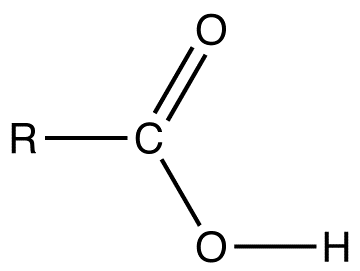
\includegraphics{carboxylic_acid.png}
\centering
\end{figure}

\section{Esters}
Esters have a pair of alkyl or aromatic groups attached to a carbonyl + linking
oxygen function.

Esters can be shown as \texttt{RCOOR}.

The reaction between a carboxylic acid and an alcohol produces an ester and
water.
This is an acid catalyzed equilibrium.

\begin{figure}[ht]
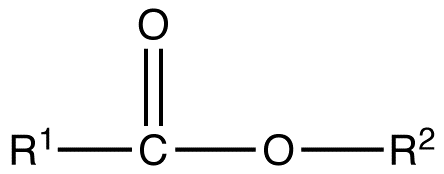
\includegraphics{ester.png}
\centering
\end{figure}

\section{Amides}
\subsection{Primary Amides}
Primary amides have an alkyl or aromatic group attached to an amino-carbonyl
function.

Primary amides can be shown as \texttt{RCONH2}.

\subsection{Secondary Amides}
Secondary amides have an alkyl or aryl group attached to the nitrogen:
\texttt{RCONHR}.

\subsection{Tertiary Amides}
Tertiary amides have two alkyl or aryl group attached to the nitrogen:
\texttt{RCONR2}.

\section{Amines}
\subsection{Primary amine}
Primary amines have an alkyl or aromatic group and two hydrogens attached to a
nitrogen atom.

Primary amines are basic functions that can be protonated to the corresponding
ammonium ion.
Primary amines are also nucleophilic.

Primary amines can be shown as \texttt{RNH2}.

\subsection{Secondary amine}
Secondary amines have a pair of alkyl or aromatic groups, and a hydrogen,
attached to a nitrogen atom.

Secondary amines are basic functions that can be protonated to the corresponding
ammonium ion.
Secondary amines are also nucleophilic.

Secondary amines can be shown as \texttt{R2NH}.

\subsection{Tertiary amine}
Tertiary amines have three alkyl or aromatic groups attached to a nitrogen atom.

Tertiary amines are basic functions that can be protonated to the corresponding
ammonium ion.
Tertiary amines are also nucleophilic.

Tertiary amines can be shown as \texttt{R3N}.

\section{Acid chlorides}
Acid chlorides, or acyl chlorides, have an alkyl (or aromatic) group attached to
a carbonyl function plus a labile (easily displaced) chlorine.

Acid chlorides highly reactive entities are highly susceptible to attack by
nucleophiles.
Acid chlorides can be shown as \texttt{RCOCl}.

\section{Acid anhydrides}
Acid anhydrides are formed when water is removed from a carboxylic acid, hence
the name.

Acid anhydrides can be shown as \texttt{(RCO)2O}.

\begin{figure}[ht]
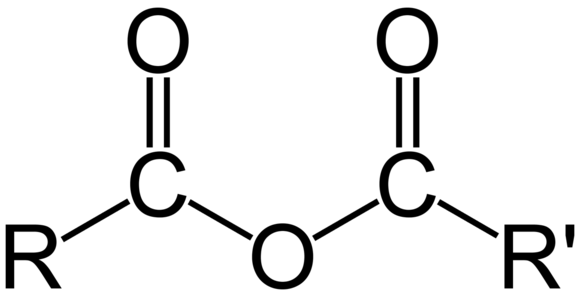
\includegraphics[scale=0.2]{carboxylic-acid-anhydride.png}
\centering
\end{figure}

\section{Nitriles}
Nitriles (or organo cyanides) have an alkyl (or aromatic) group attached to a
carbon-triple-bond-nitrogen function.

Nitriles can be shown as \texttt{RCN}.

Note that there is a nomenclature issue with nitriles/cyanides. If a compound is
named as the nitrile then the nitrile carbon is counted and included, but when
the compound is named as the cyanide it is not.

For instance, \texttt{CH3CH2CN} is called propane nitrile or ethyl cyanide
(cyanoethane).

\section{Carboxylate ion or salt}
Carboxylate ions are the conjugate bases of carboxylic acids, i.e. the
deprotonated carboxylic acid.

When the counter ion is included, the salt is being shown.

Salts can be shown as \texttt{RCOONa}.

\section{Amino Acids}
Amino acids, strictly alpha-amino acids, have carboxylic acid, amino function
and a hydrogen attached to a the same carbon atom.

There are 20 naturally occurring amino acids. All except glycine (R = H) are
chiral and only the L enantiomer is found in nature.

Amino acids can be shown as \texttt{R-CH(NH2)COOH}.

\begin{figure}[ht]
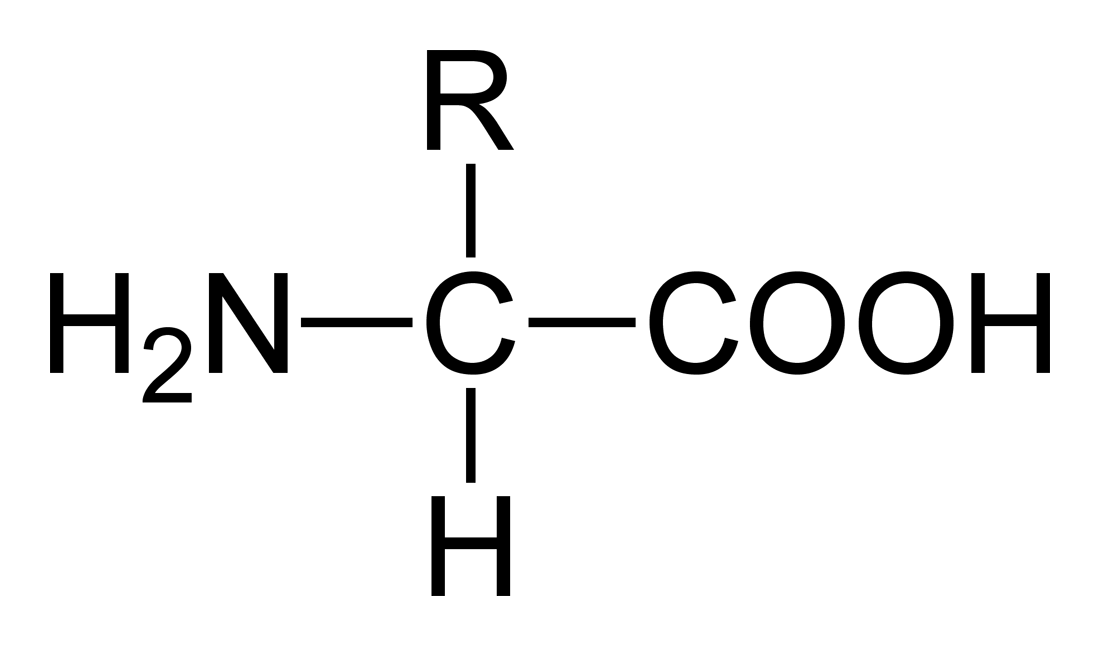
\includegraphics[scale=0.125]{alpha-amino-acid-flat.png}
\centering
\end{figure}

\section{Ethers}
Ethers have a pair of alkyl or aromatic groups attached to a linking oxygen
atom.

Ethers are surprisingly unreactive and are very useful as solvents for many many
(but not all) classes of reaction.

Ethers can be shown as \texttt{ROR}.

\section{Polymer}
Polymers consist of small monomer molecules that have reacted together so as to
form a large covalently bonded structure.

There are two general types of polymerisation: addition and condensation.

Linear chain polymers are generally thermoplastic, while three dimensional
network polymers are not. \textbf{Thermoplastic polymers} become pliable or
moldable above a specific temperature and solidify upon cooling, while
\textbf{thermosetting polymers} cure irreversibly. The cure may be induced by
heat, through a chemical reaction, or suitable irradiation. Thermoset materials
are usually liquid or malleable prior to curing and designed to be molded into
their final form, or used as adhesives. Once hardened a thermoset resin cannot
be reheated and melted to be shaped differently.

\part{Physics}

\chapter{Kinetics}
\[S = S_0 + V_0 t + \frac{a t^2}{2}\]
\[V_f^2 = V_i^2 + 2 a \Delta S\]

\chapter{Waves}
\[v = \lambda f\]

\section{Doppler Effect}
\[f = f_0 \left ( \frac{v + v_r}{v + v_s} \right )\]

where

\(v\) is the velocity of waves in the medium;

\(v_r\) is the velocity of the receiver relative to the medium; positive if the
receiver is moving towards the source (and negative in the other direction);

\(v_s\) is the velocity of the source relative to the medium; positive if the
source is moving away from the receiver (and negative in the other direction).

One can remember that the velocities are positive if the receiver is chasing
the source.

\section{Sound Intensity}
For a spherical sound wave, the intensity in the radial direction as a function
of distance \(r\) from the center of the sphere is given by

\[I(r) = \frac{P}{A(r)} = \frac{P}{4 \pi r^2}\]

\section{Pendulum}
The period of swing of a simple gravity pendulum depends on its length, the
local strength of gravity, and to a small extent on the maximum angle that the
pendulum swings away from vertical, called the amplitude. It is independent of
the mass of the bob. If the amplitude is limited to small swings, the period T
of a simple pendulum, the time taken for a complete cycle, is:
\[T \approx 2 \pi \sqrt{\frac{l}{g}}\]

\chapter{Gases}
\[P = P_A + \rho g h\]
\[\tau = P \Delta V\]

\chapter{Electricity}
\[U = R i\]
\[P = i U\]
Resistance of a parallel association of resistors:
\[\reciprocal{R_{eq}} = \sum{\reciprocal{R_i}}\]

\section{Electric Force}
\[F_{el} = \frac{k Q q}{r^2}\]

\section{Transformers}
A transformer makes use of Faraday's law and the ferromagnetic properties of an
iron core to efficiently raise or lower alternating current (AC) voltages.
For an ideal transformer, the voltage ratio is equal to the turns ratio, and
power in equals power out.

\[\frac{V_1}{V_2} = \frac{N_1}{N_2}\]

\[P_{\text{in}} = P_{\text{out}}\]

\chapter{Electromagnetism}

\section{Magnetic Force}
\[F_{mag} = B q v = B i l\]

\section{Magnetic Fields}
\[B_{\text{wire}} = \frac{i \mu_0}{2 \pi r}\]
\[B_{\text{current loop}} = \frac{i \mu_0}{2 r}\]

\section{Lenz's Law}
Lenz's law is a common way of understanding how electromagnetic circuits obey
Newton's third law and the conservation of energy.
\begin{quote}
If an induced current flows, its direction is always such that it will oppose
the change which produced it.
\end{quote}
Lenz's law is shown with the negative sign in Faraday's law of induction:
\[{E}=-\frac{\partial \Phi}{\partial t}\]

\chapter{Modern Physics}
\[E = hf = h\frac{c}{\lambda}\]

\section{Lorentz factor}
The Lorentz factor is the factor by which time, length, and relativistic mass
change for an object while that object is moving.
\[\gamma = \reciprocal{\sqrt{1 - \frac{v^2}{c^2}}}\]

\section{Superposition}
Superposition is a principle of quantum theory that describes a challenging
concept about the nature and behavior of matter and forces at the sub-atomic
level. The principle of superposition claims that while we do not know what the
state of any object is, it is actually in all possible states simultaneously,
as long as we don't look to check. It is the measurement itself that causes the
object to be limited to a single possibility. It can also be said that there is
no single outcome unless it is observed.

Superposition is well illustrated by \textbf{Thomas Young's double-slit
experiment}, developed in the early nineteenth century to prove that light
consisted of waves. Richard Feynman claimed that the essentials of quantum
mechanics could be grasped by an exploration of the implications of Young's
experiment.

In this experiment, a beam of light is aimed at a barrier with two vertical
slits.  The light passes through the slits and the resulting pattern is
recorded.  If one slit is covered, the pattern is what would be expected: a
single line of light, aligned with whichever slit is open. Intuitively, one
would expect that if both slits are open, the pattern of light will reflect
that fact: two lines of light, aligned with the slits.  However, what happens
is that the plate is entirely separated into multiple lines of lightness and
darkness in varying degrees.  What is being illustrated by this result is that
interference is taking place between the waves/particles going through the
slits, in what, seemingly, should be two non-crossing trajectories.

We would expect that if the beam of light particles or photons is slowed enough
to ensure that individual photons are hitting the plate, there could be no
interference and the pattern of light would be two lines of light, aligned with
the slits. In fact, however, the resulting pattern still indicates
interference, which means that, somehow, the single particles are interfering
with themselves. This seems impossible: we expect that a single photon will go
through one slit or the other, and will end up in one of two possible light
line areas. But that is not what happens. As Feynman concluded, each photon not
only goes through both slits, but simultaneously takes every possible
trajectory en route to the target.

In order to see how this might possibly occur, experiments have focused on
tracking the paths of individual photons. What happens in this case is that the
measurement in some way disrupts the photons' trajectories (in accordance with
the uncertainty principle), and somehow, the results of the experiment become
what would be predicted by classical physics: two bright lines on the
photographic plate, aligned with the slits in the barrier. Cease the attempt to
measure, however, and the pattern will again become multiple lines in varying
degrees of lightness and darkness. Each photon moves simultaneously in a
superposition of possible trajectories, and, furthermore, measurement of the
trajectory causes the superposition of states to collapse to a single position.

Text extracted from
\href{http://whatis.techtarget.com/definition/superposition}{WhatIs}.

\part{Mathematics}

\chapter{Set Theory}
\section{Power Set}
The power set \(P(S)\) is the set of all subsets of \(S\), including the empty
set and the set \(S\) itself.

It has \(2^n\) elements where \(n\) is the number of elements in \(S\).

\chapter{Linear Algebra}

\section{Row operations}
\begin{itemize}
\item{Replace one row by the sum of itself and a multiple of another row.}
\item{Interchange two rows.}
\item{Multiply all entries in a row by a nonzero constant.}
\end{itemize}

\section{Row equivalence}
Two matrices are \textbf{row equivalent} if, and only if, there is a sequence
of row operations that transform one matrix into another.
Row equivalence is indicated by a tilde (\(\sim\)) between matrices.
\section{Echelon form}
A matrix is in \textbf{echelon form} if it has the shape resulting from a
Gaussian
elimination.
The following are properties of the echelon matrix:
\begin{itemize}
\item{All nonzero rows are above any rows of all zeros.}
\item{The leading entry of a row is at least one column to the right of the
leading entry of the row above it.}
\end{itemize}
The following are properties of the \textbf{reduced echelon matrix}:
\begin{itemize}
\item{The leading entry in any nonzero row is 1.}
\item{Each leading 1 is the only nonzero in its column.}
\end{itemize}

\section{Row reducing algorithm}
The \textbf{forward phase} of the row reducing algorithm produces the row
echelon form.
The \textbf{backward phase} produces the unique reduced row echelon form.
Computer algorithms usually select as a pivot the entry in a column that has the
largest value.
This strategy, called partial pivoting, is used to reduce roundoff errors in the
calculations.
Computers do not perform the backward phase in order to find the reduced echelon
form, instead,
they perform back substitution.
The best strategy is to use the reduced echelon form only when solving a system
by hand.
A flop is one arithmetic operation (+, -, *, /) on two real floating point
numbers.
(Traditionally, + and - were not considered to be flops, but nowadays they are).

\section{Solution existence and uniqueness}
A solution exists if there are no invalid equations, such as \( 0 = 1 \). The
solution is unique if, and only if, there are no free variables.

\subsection{Existence and uniqueness theorem}
A system is consistent if, and only if, the rightmost column of the augmented
matrix is not a pivot column.
Stated differently, a matrix equation of the form \(A\mathbf{x} = \mathbf{b\)
has a solution if, and only if, \(\mathbf{b}\) is a linear combination of the
columns of \(\mathbf{A}\), that is, if \(\mathbf{b} \in \mathrm{Span}
\{\mathbf{a}_1, \ldots, \mathbf{a}_n\}\).

\section{Parallelogram Rule for Addition}
If \(\mathbf{u}\) and \(\mathbf{v}\) in \(\mathbb{R}^\)2
are represented as points in the plane,
then \(\mathbf{u} + \mathbf{v}\) corresponds to the fourth vertex of the
parallelogram whose other vertices are \(\mathbf{0}\), \(\mathbf{u}\) and
\(\mathbf{v}\).

\section{Linear combinations}
Given vectors \(\mathbf{v}_1, \mathbf{v}_2, \ldots, \mathbf{v}_p\) in
\(\mathbb{R}^n\) and given scalars \(c_1, c_2, \ldots, c_p\) in \(\mathbb{R}\),
the vector \(\mathbf{y}\) defined by
\[ \mathbf{y} = c_1 \mathbf{v}_1 + \ldots + c_p \mathbf{v}_p \]
is called a \textbf{linear combination} of
\(\mathbf{v}_1, \ldots, \mathbf{v}_p\) with weights \(c_1, \ldots, c_p\).

\section{Span}
The set of all linear combinations of \(\mathbf{v}_1, \ldots, \mathbf{v}_p\) in
\(\mathbb{R}^n\) is called the \textbf{subset of \(\mathbb{R}^n\) spanned (or






generated) by 010\mathbf{v}_1, \ldots, \mathbf{v}_p010} and is denoted by
010\mathrm{Span}\{\mathbf{v}_1, \ldots, \mathbf{v}_p\}020. If a matrix 010A020 has a
pivot in every row, then 010\mathrm{Span} \{\mathbf{a}_1, \ldots, \mathbf{a}_n\}
= \mathbb{R}^m020.

\end{document}
